\documentclass{beamer}
\usepackage{etex}
\usepackage[utf8]{inputenc}
\usepackage[T1]{fontenc}
\usepackage{amssymb}
\usepackage{color}
\usepackage{verbatim}
\usepackage{beamerthemesplit}
\usepackage{graphicx}
\usepackage{xspace}
\usepackage{algorithm}
\usepackage{listings}
\usepackage{figlatex}
\usepackage{algorithmic}
\usepackage{multirow}
%\usepackage{appendixnumberbeamer}

\graphicspath{{fig/}{campagne/fig}}
\newcommand{\talk}[2]{{#1} dit : {#2}}
\newcommand{\erik}[1]{\talk{Erik}{#1}}
\newcommand{\brice}[1]{\talk{Brice}{#1}}
\beamertemplatetransparentcovereddynamic

%\setbeamertemplate{background canvas}[vertical shading][bottom=red!10,top=blue!10]
%\usetheme{Warsaw}

\usepackage{../style/beamercolorthemeprogressbar}
\usepackage{../style/beamerfontthemeprogressbar}
\usepackage{../style/beamerouterthemeprogressbar}
\usepackage{../style/beamerinnerthemeprogressbar}

\newcommand{\bordereau}{Bordereau\xspace}
\newcommand{\genepi}{Genepi\xspace}
\newcommand{\minelement}{{\em min\_element}\xspace}
\newcommand{\stablesort}{{\em stable\_sort}\xspace}
\newcommand{\merge}{{\em merge}\xspace}
\newcommand{\sort}{{\em sort}\xspace}
\newcommand{\find}{{\em find}\xspace}
\setbeamertemplate{navigation symbols}{}
\beamertemplatetransparentcovereddynamic
\newcommand{\pastel}{PaSTeL\xspace}

\definecolor{javared}{rgb}{0.6,0,0} % for strings
\definecolor{javagreen}{rgb}{0.30,0.55,0.40} % comments
\definecolor{javapurple}{rgb}{0.5,0,0.35} % keywords
\definecolor{javadocblue}{rgb}{0.25,0.35,0.75} % java

\lstdefinestyle{BOAST}{
  language=Ruby,
  basicstyle=\tiny\ttfamily,
  keywordstyle=\color{javapurple}\bfseries,
  stringstyle=\color{javared},
  commentstyle=\color{javagreen},
  backgroundcolor=\color{white},
  morekeywords={BOAST, pr, decl, opn, close}
}
\lstdefinestyle{C}{
language=C,
basicstyle=\ttfamily,
keywordstyle=\color{javapurple}\bfseries,
stringstyle=\color{javared},
commentstyle=\color{javagreen},
numbers=left,
tabsize=4,
showspaces=false,
showstringspaces=false}

\lstdefinestyle{CL}{
language=C,
basicstyle=\ttfamily,
keywordstyle=\color{javapurple}\bfseries,
stringstyle=\color{javared},
commentstyle=\color{javagreen},
morekeywords={kernel, global, uchar, uchar16, int16, short16},
numbers=left,
tabsize=4,
showspaces=false,
showstringspaces=false}

\lstdefinestyle{Fortran}{
language=Fortran,
basicstyle=\ttfamily,
keywordstyle=\color{javapurple}\bfseries,
stringstyle=\color{javared},
commentstyle=\color{javagreen},
numbers=left,
tabsize=4,
showspaces=false,
showstringspaces=false}

\lstdefinestyle{Bash}{
language=Bash,
basicstyle=\ttfamily,
keywordstyle=\color{javapurple}\bfseries,
stringstyle=\color{javared},
commentstyle=\color{javagreen},
numbers=left,
tabsize=4,
showspaces=false,
showstringspaces=false}

\graphicspath{{../figures/}}

\title{BOAST}
\subtitle{Performance Portability Using Meta-Programming and Auto-Tuning}
\author[B. V.]{\textbf{Brice~Videau}~\inst{1}, Kevin~Pouget~\inst{1}, Luigi~Genovese~\inst{2},
                    Thierry~Deutsch~\inst{2}, Dimitri~Komatitsch~\inst{3}, Jean-François~Méhaut~\inst{1}}
\institute[INRIA]{\inst{1} INRIA - Corse, \inst{2} CEA - L\_Sim, \inst{3} CNRS}

\date{\textbf{EoCoE Kickoff Meeting}\\October 5, 2015}

\begin{document}

\frame{\titlepage}

\section{Introduction}

\subsection{Context}

\begin{frame}
  \frametitle{Scientific Application Portability}

  \begin{block}{\footnotesize Limited Portability}
    \begin{itemize}
      \item \scriptsize Huge codes (more than 100 000 lines), Written in FORTRAN or C++
      \item \scriptsize Collaborative efforts
      \item \scriptsize Use many different programing paradigms
    \end{itemize}
  \end{block}

  \begin{columns}

  \column{0.45\linewidth}
  \begin{block}{\footnotesize But Based on \emph{Computing Kernels}}
    \begin{itemize}
      \item \scriptsize Well defines part of a program
      \item \scriptsize Compute intensive
      \item \scriptsize Prime target for optimization
    \end{itemize}
  \end{block}

  \column{0.58\linewidth}
  \begin{block}{\footnotesize Kernels Should Be Written:}
    \begin{itemize}
      \item \scriptsize In a \emph{portable} manner
      \item \scriptsize In a way that raises developer \emph{productivity}
      \item \scriptsize To present good \emph{performance}
    \end{itemize}
  \end{block}

  \end{columns}

\end{frame}

\begin{frame}
  \frametitle{HPC Architecture Evolution}

  \begin{columns}

  \column{0.6\linewidth}
  \begin{block}{\footnotesize Very Rapid and Diverse, Top500:}
    \begin{itemize}
      \item \scriptsize Intel processor + Xeon Phi (Tianhe-2)
      \item \scriptsize AMD processor + nVidia GPU (Titan)
      \item \scriptsize IBM BlueGene/Q (Sequoia)
      \item \scriptsize Fujitsu SPARC64 (K Computer)
      \item \scriptsize Intel processor + nVidia GPU (Tianhe-1)
      \item \scriptsize AMD processor (Jaguar)
    \end{itemize}
  \end{block}

  \column{0.4\linewidth}
  \begin{block}{\footnotesize Tomorrow?}
    \begin{itemize}
      \item \scriptsize ARM + DSP?
      \item \scriptsize Intel Atom + FPGA?
      \item \scriptsize Quantum computing?
    \end{itemize}
  \end{block}

  \end{columns}

  \vspace{1cm}
  How to write kernels that could adapt to those architectures?\\
  (well maybe not quantum computing...)

\end{frame}


\subsection{Case Study}

\begin{frame}
    \frametitle{BigDFT a Tool for Nanotechnologies}
Ab initio simulation:
\begin{columns}
\column{6cm}
\begin{itemize}
  \item Simulates the properties of crystals and molecules,
  \item Computes the electronic density,
  \item Based on Daubechie wavelet.
\end{itemize}
The formalism was chosen because it is fit for HPC computations: 
\begin{itemize}
\item Each orbital can be treated independently most of the time,
\item Operator on orbitals are simple and straightforward.
\end{itemize}
\column{4.5cm}
\centering
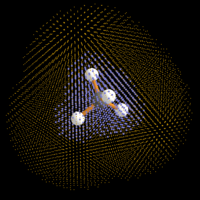
\includegraphics[width=3.5cm]{CH4-grid.png}\\
Electronic density around a methane molecule.
\end{columns}
\end{frame}


\begin{frame}
  \frametitle{3D convolutions}
  Operators can be expressed as 3D convolutions :
  \begin{itemize}
    \item Wavelet Transform
    \item Potential Energy
    \item Kinetic Energy
  \end{itemize}
  These convolutions are separable and filter are short (around 16 elements).\\
  Can take up to 80\% of the computation time on some systems.
\end{frame}

\begin{frame}[fragile]
\frametitle{Case Study: the MagicFilter}
The simplest convolution found in BigDFT, corresponds to the potential operator.
\begin{columns}
\column{4cm}
\begin{block}{Characteristics}
\begin{itemize}
\item Separable,
\item Filter length 16,
\item Transposition,
\item Periodic,
\item Only 32 operations per element.
\end{itemize}
\end{block}
\column{6.2cm}
\begin{block}{Pseudo code}
\tiny
\lstset{style=C}
\begin{lstlisting}
double filt[16] = {F0, F1, ... , F15};
void magicfilter(int n, int ndat, 
                 double *in, double *out){
  double temp;
  for(j=0; j<ndat; j++) {
    for(i=0; i<n; i++) {
       temp = 0;
       for(k=0; k<16; k++) {
         temp+= in[ ((i-7+k)%n) + j*n] 
                  * filt[k];
       }
       out[j + i*ndat] = temp;
} } }
\end{lstlisting}
\end{block}
\end{columns}
\end{frame}

\begin{frame}
    \frametitle{Talk Outline}
    \tableofcontents[hideallsubsections,sections={2-}]
    %\includegraphics{plan_couleur.pdf}
\end{frame}

\section{A Parametrized Generator}

\begin{frame}

  \frametitle{Classical Tuning of Computing Kernels}

  \begin{center}%
    \includegraphics<1>[scale=1]{Workflow1-1}%
    \includegraphics<2>[scale=1]{Workflow1-2}%
    \includegraphics<3>[scale=1]{Workflow1-3}%
    \includegraphics<4>[scale=1]{Workflow1-4}%
  \end{center}%
  \begin{itemize}%
\only<1>{    \item Kernel optimization workflow}%
\only<1>{    \item Usually performed by a knowledgeable developer}%
\only<2>{    \item Compilers perform optimizations}%
\only<2>{    \item Architecture specific or generic optimizations}%
\only<3>{    \item Performance data hint at source transformations}%
\only<3>{    \item Architecture specific or generic hints}%
\only<4>{    \item Multiplication of kernel versions or loss of versions}%
\only<4>{    \item Difficulty to benchmark versions against each-other}%
  \end{itemize}%

\end{frame}

\begin{frame}
  \frametitle{BOAST Workflow \vphantom{Cp}}
  \begin{center}
    \includegraphics<1>[scale=1]{Workflow2-1}
    \includegraphics<2>[scale=1]{Workflow2-2}
    \includegraphics<3>[scale=1]{Workflow2-3}
  \end{center}
  \begin{itemize}%
\only<1>{    \item Meta-programming of optimizations in BOAST }
\only<1>{    \item High level object oriented language }
\only<2>{    \item Generate combination of optimizations }
\only<2>{    \item C, OpenCL, FORTRAN and CUDA are supported }
\only<3>{    \item Compilation and analysis are automated }
\only<3>{    \item Selection of best version can also be automated \vphantom{Cp}}
  \end{itemize}%
\end{frame}

\begin{frame}
\frametitle{BOAST Architecture}
 \begin{center}
   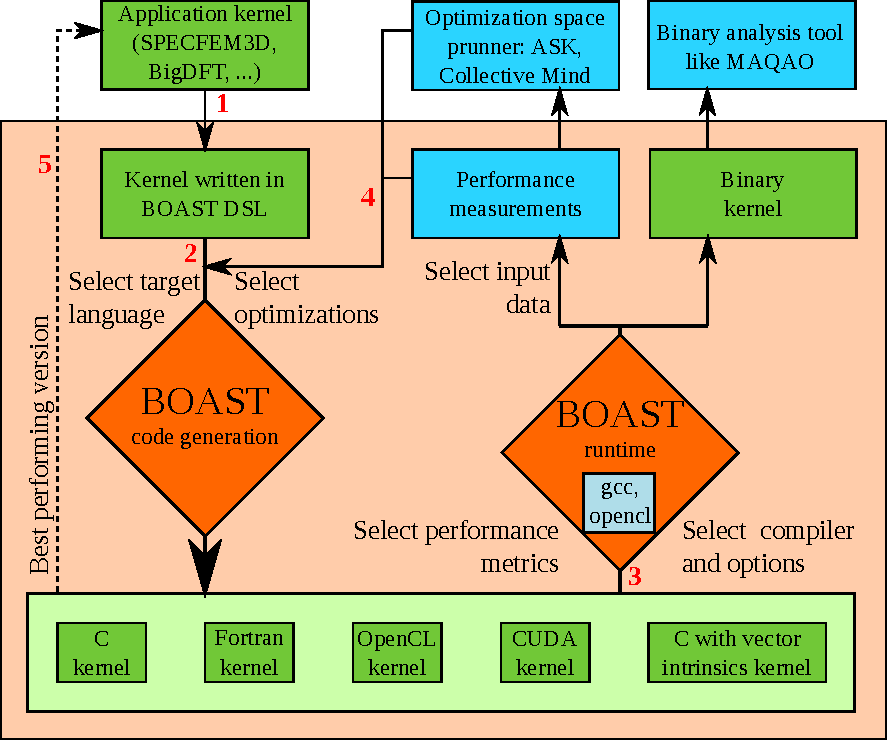
\includegraphics[scale=0.5]{BOAST_Workflow}
 \end{center}
\end{frame}

\begin{frame}
  \frametitle{Back to the use case: BigDFT}
Parameters arising in a convolution:
\begin{itemize}
\item Filter: length, values, center.
\item Direction: forward or inverse convolution.
\item Boundary conditions: free or periodic.
\item Unroll factor: arbitrary.
\end{itemize}
How are those parameters constraining our tool?
\end{frame}

\begin{frame}
\frametitle{Features required}
Unroll factor:
\begin{itemize}
\item Create an arbitrary number of temporary variables,
\item Create loops with variable steps.
\end{itemize}
Boundary conditions:
\begin{itemize}
\item Manage arrays with parametrized size.
\end{itemize}
Filter and convolution direction:
\begin{itemize}
\item Transform arrays.
\end{itemize}
And of course be able to describe convolutions and output them in different languages.
\end{frame}

\begin{frame}
\frametitle{Proposed Generator}
Idea: use a high level language with support for operator overloading to describe the structure of the code, rather than trying to transform a decorated tree.\\
Define several abstractions:
\begin{itemize}
\item Variables: type (array, float, integer), size...
\item Operators: affect, multiply...
\item Procedure and functions: parameters, variables...
\item Constructs: if, case, for, while...
\end{itemize}
\end{frame}

\begin{frame}[fragile]
\frametitle{Sample Code: Variables and Parameters}
\tiny
%\lstset{language=Ruby,numbers=left}
\lstset{style=BOAST}
\begin{lstlisting}
  #simple Variable
  i = Int("i")
  #simple constant
  lowfil = Int("lowfil", :constant => 1-center)
  #simple constant array
  fil = Real("fil", :const => arr,
                    :dim => [ Dim(lowfil,upfil) ])
  #simple parameter
  ndat = Int("ndat", :direction => :in)
  #multidimensional array, an output parameter
  y = Real("y", :dir => :out, 
                :dim => [ Dim(ndat), 
                          Dim(dim_out_min, dim_out_max) ] )
\end{lstlisting}
\normalsize
Variables and Parameters are objects with a name, a type, and a set of named properties.
\end{frame}

\begin{frame}[fragile]
\frametitle{Sample Code: Procedure Declaration}
The following declaration:
\tiny
\lstset{style=BOAST}
\begin{lstlisting}
p = Procedure("magic_filter", [n,ndat,x,y], :constants => [lowfil,upfil])
opn p
close p
\end{lstlisting}
\normalsize 
Outputs Fortran:
\tiny
\lstset{style=Fortran}
\begin{lstlisting}
SUBROUTINE magicfilter(n, ndat, x, y)
  integer(kind=4), parameter :: lowfil = -8
  integer(kind=4), parameter :: upfil = 7
  integer(kind=4), intent(in) :: n
  integer(kind=4), intent(in) :: ndat
  real(kind=8), intent(in), dimension(0:n-1, ndat) :: x
  real(kind=8), intent(out), dimension(ndat, 0:n-1) :: y
END SUBROUTINE magicfilter
\end{lstlisting}
\normalsize
Or C:
\tiny
\lstset{style=C}
\begin{lstlisting}
void magicfilter(const int32_t n, const int32_t ndat, const double * x, double * y){
  const int32_t lowfil = -8;
  const int32_t upfil = 7;
}
\end{lstlisting}
\end{frame}

\begin{frame}[fragile]
\frametitle{Sample Code: Constructs and Arrays}
The following declaration:
\tiny
\lstset{style=BOAST}
\begin{lstlisting}
  unroll = 5
  tt = (0...unroll).collect { |t| Real("tt#{t}") }
  pr For(j, 1, ndat-(unroll-1), unroll){
    pr For( i, 0, n-1) {
      (0...unroll).each { |u| pr tt[u] === 0 }
      For(l, -8, 7) {
        pr k === modulo(i + l, n)
        (0...unroll).each { |u|
          pr tt[u] === tt[u] + x[k,j+u]*fil[l]
        }
      }.unroll
      (0...unroll).each { |u| pr y[j+u,i] === tt[u] }
    }
  }
\end{lstlisting}
\begin{columns}

\column{0.40\linewidth}
\normalsize 
Outputs Fortran:
\tiny
\lstset{style=Fortran}
\begin{lstlisting}
  do j=1, ndat-4, 5
    do i=0, n-1
      !......
      k = modulo(i+2, n)
      tt0=tt0+x(k,j+0)*fil(2)
      tt1=tt1+x(k,j+1)*fil(2)
      !......
    enddo
  enddo
\end{lstlisting}
\column{0.60\linewidth}
\normalsize
Or C:
\tiny
\lstset{style=C}
\begin{lstlisting}
  for(j=1; j<=ndat-4; j+=5){
    for(i=0; i<=n-1; i+=1){
  /*...........*/
      k = modulo(i+2, n)
      tt0=tt0+x[k-0+(j+0-1)*(n-1-0+1)]*fil[2-lowfil];
      tt1=tt1+x[k-0+(j+1-1)*(n-1-0+1)]*fil[2-lowfil];
  /*...........*/
    }
  }
\end{lstlisting}
\end{columns}
\end{frame}

\section{Evaluation}
\begin{frame}
\frametitle{Generator Evaluation}

\end{frame}

\begin{frame}
\frametitle{BigDFT: Magicfilter}
The generator was used to unroll the Magicfilter an evaluate it's performance on an ARM processor and an Intel processor.
\centering
\begin{columns}
\column{5cm}
\begin{block}{Tegra2}
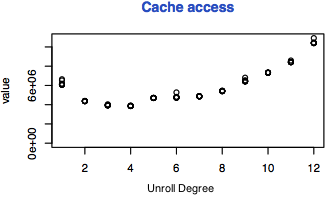
\includegraphics[scale=0.4]{cacc}\\
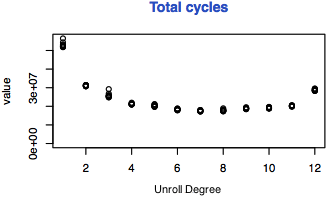
\includegraphics[scale=0.4]{totcyc}
\end{block}
\column{5cm}
\begin{block}{Intel T7500}
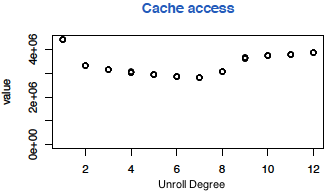
\includegraphics[scale=0.4]{nedni_cacc.png}\\
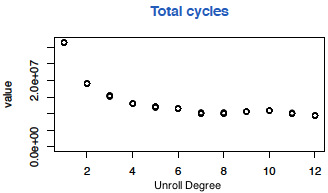
\includegraphics[scale=0.4]{nedni_totcyc.png}
\end{block}
\end{columns}
\end{frame}


\begin{frame}
  \frametitle{BigDFT: Synthesis}
  \begin{center}
    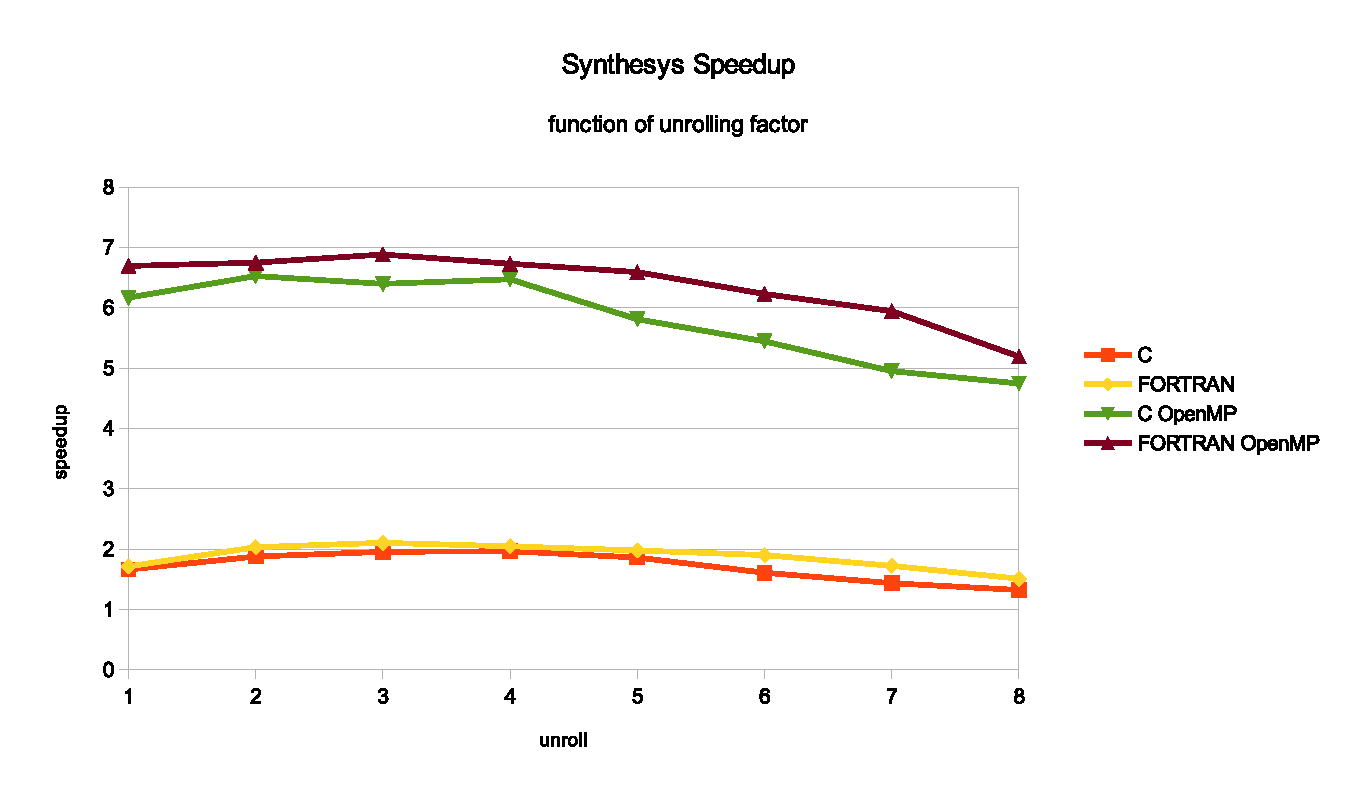
\includegraphics[scale=0.40]{Res_synthesis}
  \end{center}

  \begin{itemize}
    \item Reference is hand tuned code on target architecture
    \item Toward a BLAS-like library fo wavelets
  \end{itemize}
\end{frame}


\begin{frame}[fragile]
  \frametitle{Example: Laplace Kernel from ARM}
\tiny
\lstset{style=C}
\begin{lstlisting}
void laplace(const int width,
             const int height,
             const unsigned char src[height][width][3],
                   unsigned char dst[height][width][3]){
  for (int j = 1; j < height-1; j++) {
    for (int i = 1; i < width-1; i++) {
      for (int c = 0; c < 3; c++) {
        int tmp = -src[j-1][i-1][c] -   src[j-1][i][c] - src[j-1][i+1][c]\
                 - src[j  ][i-1][c] + 9*src[j  ][i][c] - src[j  ][i+1][c]\
                 - src[j+1][i-1][c] -   src[j+1][i][c] - src[j+1][i+1][c];
        dst[j][i][c] = (tmp < 0 ? 0 : (tmp > 255 ? 255 : tmp));
      }
    }
  }
}
\end{lstlisting}
\begin{itemize}
\item C reference implementation
\item Many opportunities for improvement
\end{itemize}
\end{frame}

\begin{frame}
  \frametitle{Example: Optimization Summary}
  \begin{itemize}
    \item Very complex process
    \item Intimate knowledge of the architecture required
    \item Numerous versions to be benchmarked
    \item Difficult to test combination of optimizations:
    \begin{itemize}
      \item Vectorization,
      \item Intermediary data type,
      \item Number of pixels processed,
      \item Synthesizing loads.
    \end{itemize}
    \item Can we use BOAST to automate the process?
  \end{itemize}
\end{frame}

\begin{frame}
  \frametitle{Example: Laplace Kernel with BOAST}
  \begin{itemize}
    \item Based on components instead of pixel
    \item Use tiles rather than only sequence of elements
    \item Parameters used in the BOAST version:
    \begin{itemize}
      \item \emph{x\_component\_number}: a positive integer
      \item \emph{y\_component\_number}: a positive integer
      \item \emph{vector\_length}: 1, 2, 4, 8 or 16
      \item \emph{temporary\_size}: 2 or 4
      \item \emph{synthesizing\_loads}: true or false
    \end{itemize}
  \end{itemize}
\end{frame}

\begin{frame}
  \frametitle{Example: ARM results}
  \begin{center}
  \scriptsize
  \begin{tabular}{c|r|r|c|r|c}
    Image Size  & Naive (s) & Best (s) & Acceleration & BOAST (s) & Acceleration \\
    \hline&&&&\\
  768 x 432   & 0.0107    & 0.00669  & x1.6         & 0.000639  & x16.7 \\
  2560 x 1600 & 0.0850    & 0.0137   & x6.2         & 0.00687   & x12.4 \\
  2048 x 2048 & 0.0865    & 0.0149   & x5.8         & 0.00715   & x12.1 \\
  5760 x 3240 & 0.382     & 0.0449   & x8.5         & 0.0325    & x11.8 \\
  7680 x 4320 & 0.680     & 0.0747   & x9.1         & 0.0581    & x11.7
  \end{tabular}
  \end{center}

  \begin{itemize}
    \item Optimal parameter values:
    \begin{itemize}
      \item x\_component\_number: 16
      \item y\_component\_number: 1
      \item vector\_length: 16
      \item temporary\_size: 2
      \item synthesizing\_loads: false
    \end{itemize}
    \item Close to what ARM engineers found
  \end{itemize}
\end{frame}

\begin{frame}
  \frametitle{Example: Performance Portability}
  \begin{center}
  \scriptsize
  \begin{tabular}{c|r|r|c|r|c}
    Image Size & BOAST ARM (s) & BOAST Intel & Ratio & BOAST NVIDIA & Ratio \\
    \hline&&&&\\
  768 x 432   & 0.000639     & 0.000222    & x2.9  & 0.0000715    & x8.9  \\
  2560 x 1600 & 0.00687      & 0.00222     & x3.1  & 0.000782     & x8.8  \\
  2048 x 2048 & 0.00715      & 0.00226     & x3.2  & 0.000799     & x8.9  \\
  5760 x 3240 & 0.0325       & 0.0108      & x3.0  & 0.00351      & x9.3  \\
  7680 x 4320 & 0.0581       & 0.0192      & x3.0  & 0.00623      & x9.3
  \end{tabular}
  \end{center}

  \begin{columns}
  \column{0.5\textwidth}
  \begin{itemize}
    \item \footnotesize Optimal parameter values Intel:
    \begin{itemize}
      \item \scriptsize x\_component\_number: 16
      \item \scriptsize y\_component\_number: 4..2
      \item \scriptsize vector\_length: 8
      \item \scriptsize temporary\_size: 2
      \item \scriptsize synthesizing\_loads: false
    \end{itemize}
  \end{itemize}
  \column{0.5\textwidth}
  \begin{itemize}
    \item \footnotesize Optimal parameter values nVidia:
    \begin{itemize}
      \item \scriptsize x\_component\_number: 4
      \item \scriptsize y\_component\_number: 4
      \item \scriptsize vector\_length: 4
      \item \scriptsize temporary\_size: 2
      \item \scriptsize synthesizing\_loads: false
    \end{itemize}
  \end{itemize}
  \end{columns}
  \vspace{1cm}
  \centering Performance \emph{portability} among several different architectures.
\end{frame}

\begin{frame}
  \frametitle{Real Applications: SPECFEM3D}

  \begin{itemize}
    \item SPECFEM3D ported to OpenCL using BOAST
    \begin{itemize}
      \item Unified code base (CUDA/OpenCL)
      \item Refactoring: kernel code base reduced by 40\%
      \item Similar performance on NVIDIA Hardware
      \item Non regression test for GPU kernels
    \end{itemize}
    \item On the Mont-Blanc prototype:
    \begin{itemize}
      \item OpenCL+MPI runs
      \item Speedup of 3 for the GPU version
    \end{itemize}
  \end{itemize}
\end{frame}

\section{Using BOAST}

\begin{frame}[fragile]

    \frametitle{Installing BOAST}

Install ruby, version >= 1.9.3\\
On recent debian-based distributions:
\lstset{style=Bash}
\begin{lstlisting}
sudo apt-get install ruby ruby-dev
\end{lstlisting}
And then install the BOAST gem (ruby module):
\begin{lstlisting}
sudo gem install BOAST
\end{lstlisting}
If on a cluster frontend:
\begin{lstlisting}
gem install --user-install BOAST
\end{lstlisting}

\end{frame}

\begin{frame}[fragile]
\frametitle{First interactive steps}
Interactive Ruby:
\lstset{style=Bash}
\begin{lstlisting}
irb
\end{lstlisting}
Simple BOAST commands:
\lstset{style=BOAST}
\begin{lstlisting}
irb(main):001:0> require 'BOAST'
=> true
irb(main):002:0> a = BOAST::Int "a"
=> a
irb(main):003:0> b = BOAST::Real "b"
=> b
irb(main):004:0> BOAST::decl a, b
integer(kind=4) :: a
real(kind=8) :: b
=> [a, b]
\end{lstlisting}
\end{frame}

\begin{frame}[fragile]
\frametitle{Creating a Computing Kernel}
\lstset{style=BOAST}
\tiny
\begin{lstlisting}
n = BOAST::Int(  "n", :dir => :in )
a = BOAST::Real( "a", :dir => :in,  :dim => [BOAST::Dim(n)] )
b = BOAST::Real( "b", :dir => :out, :dim => [BOAST::Dim(n)] )
p = BOAST::Procedure( "test_proc", [n, a, b] ) {
  BOAST::decl i = BOAST::Int( "i" )
  BOAST::pr BOAST::For( i, 1, n ) {
    BOAST::pr b[i] === a[i] + 2
  }
}
k = BOAST::CKernel::new
BOAST::pr p
k.procedure = p
k.build
BOAST::verbose = true
k.build
> gcc -O2 -Wall -fPIC -I/usr/lib/ruby/1.9.1/x86_64-linux -I/usr/include/ruby-1.9.1 -I/usr/include/ruby-1.9.1/x86_64-linux -I/var/lib/gems/1.9.1/gems/narray-0.6.0.9 -DHAVE_NARRAY_H -c -o /tmp/Mod_test_proc20140624_19378_1qdep6u.o /tmp/Mod_test_proc20140624_19378_1qdep6u.c
> gfortran -O2 -Wall -fPIC -c -o /tmp/test_proc20140624-19378-1qdep6u.o /tmp/test_proc20140624-19378-1qdep6u.f90
> gcc -shared -o /tmp/Mod_test_proc20140624_19378_1qdep6u.so /tmp/Mod_test_proc20140624_19378_1qdep6u.o /tmp/test_proc20140624-19378-1qdep6u.o -Wl,-Bsymbolic-functions -Wl,-z,relro -rdynamic -Wl,-export-dynamic -L/usr/lib -lruby-1.9.1 -lrt
\end{lstlisting}
\end{frame}

\begin{frame}[fragile]
\frametitle{Running a Computing Kernel}
\lstset{style=BOAST}
\tiny
\begin{lstlisting}
require 'narray'
n = BOAST::Int(  "n", :dir => :in )
a = BOAST::Real( "a", :dir => :in,  :dim => [BOAST::Dim(n)] )
b = BOAST::Real( "b", :dir => :out, :dim => [BOAST::Dim(n)] )
p = BOAST::Procedure( "test_proc", [n, a, b] ) {
  BOAST::decl i = BOAST::Int( "i" )
  BOAST::pr BOAST::For( i, 1, n ) {
    BOAST::pr b[i] === a[i] + 2
  }
}
k = BOAST::CKernel::new
BOAST::pr p
k.procedure = p

input  = NArray.float(1024).random
output = NArray.float(1024)
k.run(input.length, input, output)
(output - input).each { |val|
  raise "Error!" if (val-2).abs > 1e-15
}
stats = k.run(input.length, input, output)
puts "#{stats[:duration]} s"
> 4.911e-06 s
\end{lstlisting}
\end{frame}


\section{Conclusions}

\begin{frame}
  \frametitle{Conclusions}
  \begin{itemize}
    \item BOAST v1.0 is released
    \item BOAST language features:
    \begin{itemize}
      \item Unified C and FORTRAN with OpenMP support,
      \item Unified OpenCL and CUDA support,
      \item Support for vector programming.
    \end{itemize}
    \item BOAST runtime features:
    \begin{itemize}
      \item Generation of parametric kernels,
      \item Parametric compilation,
      \item Non-regression testing of kernels,
      \item Benchmarking capabilities (PAPI support)
    \end{itemize}
  \end{itemize}
\end{frame}

\begin{frame}
  \frametitle{Perspectives}
  \begin{itemize}
    \item Find and port new kernels to BOAST
    \item Couple BOAST with other tools:
    \begin{itemize}
      \item Parametric space pruners (speed up optimization),
      \item Binary analysis (guide optimization),
      \item Source to source transformation (improve optimization),
      \item Binary transformation (improve optimization).
    \end{itemize}
    \item Improve BOAST:
    \begin{itemize}
      \item Improve the eDSL to make it more intuitive,
      \item Better vector support,
      \item Gather feedback.
    \end{itemize}
  \end{itemize}
\end{frame}

\appendix

\newcounter{finalframe}
\setcounter{finalframe}{\value{framenumber}}

\begin{frame}
  \frametitle{Question?}
\end{frame}

% Backup frames


\begin{frame}[fragile]
  \frametitle{Example: Laplace in OpenCL}
\tiny
\lstset{style=CL}
\begin{lstlisting}
kernel laplace(const int width,
               const int height,
               global const uchar *src,
               global       uchar *dst){
  int i = get_global_id(0);
  int j = get_global_id(1);
  for (int c = 0; c < 3; c++) {
    int tmp = -src[3*width*(j-1) + 3*(i-1) + c]\
             - src[3*width*(j-1) + 3*(i  ) + c]\
             - src[3*width*(j-1) + 3*(i+1) + c]\
             - src[3*width*(j  ) + 3*(i-1) + c]\
           + 9*src[3*width*(j  ) + 3*(i  ) + c]\
             - src[3*width*(j  ) + 3*(i+1) + c]\
             - src[3*width*(j+1) + 3*(i-1) + c]\
             - src[3*width*(j+1) + 3*(i  ) + c]\
             - src[3*width*(j+1) + 3*(i+1) + c];
    dst[3*width*j + 3*i + c] = clamp(tmp, 0, 255);
  }
}
\end{lstlisting}
\begin{itemize}
\item OpenCL reference implementation
\item Outer loops mapped to threads
\end{itemize}
\end{frame}

\begin{frame}[fragile]
  \frametitle{Example: Vectorizing}
\lstset{style=CL}
\fontsize{3}{3}\selectfont
\begin{lstlisting}
kernel laplace(const int width,
               const int height,
               global const uchar *src,
               global       uchar *dst){
  int i = get_global_id(0);
  int j = get_global_id(1);
  uchar16 v11_ = vload16( 0, src + 3*width*(j-1) + 3*5*i - 3 );
  uchar16 v12_ = vload16( 0, src + 3*width*(j-1) + 3*5*i     );
  uchar16 v13_ = vload16( 0, src + 3*width*(j-1) + 3*5*i + 3 );
  uchar16 v21_ = vload16( 0, src + 3*width*(j  ) + 3*5*i - 3 );
  uchar16 v22_ = vload16( 0, src + 3*width*(j  ) + 3*5*i     );
  uchar16 v23_ = vload16( 0, src + 3*width*(j  ) + 3*5*i + 3 );
  uchar16 v31_ = vload16( 0, src + 3*width*(j+1) + 3*5*i - 3 );
  uchar16 v32_ = vload16( 0, src + 3*width*(j+1) + 3*5*i     );
  uchar16 v33_ = vload16( 0, src + 3*width*(j+1) + 3*5*i + 3 );
  int16 v11 = convert_int16(v11_);
  int16 v12 = convert_int16(v12_);
  int16 v13 = convert_int16(v13_);
  int16 v21 = convert_int16(v21_);
  int16 v22 = convert_int16(v22_);
  int16 v23 = convert_int16(v23_);
  int16 v31 = convert_int16(v31_);
  int16 v32 = convert_int16(v32_);
  int16 v33 = convert_int16(v33_);
  int16 res = v22 * (int)9 - v11 - v12 - v13 - v21 - v23 - v31 - v32 - v33;
        res = clamp(res, (int16)0, (int16)255);
  uchar16 res_ = convert_uchar16(res);
  vstore8(res_.s01234567, 0, dst + 3*width*j + 3*5*i);
  vstore8(res_.s89ab,     0, dst + 3*width*j + 3*5*i + 8);
  vstore8(res_.scd,       0, dst + 3*width*j + 3*5*i + 12);
  dst[3*width*j + 3*5*i + 14] = res_.se;
}
\end{lstlisting}
\begin{itemize}
\item Vectorized OpenCL implementation
\item 5 pixels (15 compoenets)
\end{itemize}
\end{frame}

\begin{frame}[fragile]
  \frametitle{Example: Synthesizing Vectors}
\lstset{style=CL}
\tiny
\begin{lstlisting}
uchar16 v11_ = vload16( 0, src + 3*width*(j-1) + 3*5*i - 3 );
uchar16 v12_ = vload16( 0, src + 3*width*(j-1) + 3*5*i     );
uchar16 v13_ = vload16( 0, src + 3*width*(j-1) + 3*5*i + 3 );
uchar16 v21_ = vload16( 0, src + 3*width*(j  ) + 3*5*i - 3 );
uchar16 v22_ = vload16( 0, src + 3*width*(j  ) + 3*5*i     );
uchar16 v23_ = vload16( 0, src + 3*width*(j  ) + 3*5*i + 3 );
uchar16 v31_ = vload16( 0, src + 3*width*(j+1) + 3*5*i - 3 );
uchar16 v32_ = vload16( 0, src + 3*width*(j+1) + 3*5*i     );
uchar16 v33_ = vload16( 0, src + 3*width*(j+1) + 3*5*i + 3 );
\end{lstlisting}
\normalsize
\centering Becomes
\tiny
\begin{lstlisting}
uchar16 v11_ = vload16( 0, src + 3*width*(j-1) + 3*5*i - 3 );
uchar16 v13_ = vload16( 0, src + 3*width*(j-1) + 3*5*i + 3 );
uchar16 v12_ = uchar16( v11_.s3456789a, v13_.s56789abc );
uchar16 v21_ = vload16( 0, src + 3*width*(j  ) + 3*5*i - 3 );
uchar16 v23_ = vload16( 0, src + 3*width*(j  ) + 3*5*i + 3 );
uchar16 v22_ = uchar16( v21_.s3456789a, v23_.s56789abc );
uchar16 v31_ = vload16( 0, src + 3*width*(j+1) + 3*5*i - 3 );
uchar16 v33_ = vload16( 0, src + 3*width*(j+1) + 3*5*i + 3 );
uchar16 v32_ = uchar16( v31_.s3456789a, v33_.s56789abc );
\end{lstlisting}
\begin{itemize}
\item Synthesizing loads should save bandwidth
\item Could be pushed further
\end{itemize}
\end{frame}

\begin{frame}[fragile]
  \frametitle{Example: Reducing Variable Size}
\lstset{style=CL}
\tiny
\begin{lstlisting}
int16 v11 = convert_int16(v11_);
int16 v12 = convert_int16(v12_);
int16 v13 = convert_int16(v13_);
int16 v21 = convert_int16(v21_);
int16 v22 = convert_int16(v22_);
int16 v23 = convert_int16(v23_);
int16 v31 = convert_int16(v31_);
int16 v32 = convert_int16(v32_);
int16 v33 = convert_int16(v33_);
int16 res = v22 * (int)9 - v11 - v12 - v13 - v21 - v23 - v31 - v32 - v33;
      res = clamp(res, (int16)0, (int16)255);
\end{lstlisting}
\normalsize
\centering Becomes
\tiny
\begin{lstlisting}
short16 v11 = convert_short16(v11_);
short16 v12 = convert_short16(v12_);
short16 v13 = convert_short16(v13_);
short16 v21 = convert_short16(v21_);
short16 v22 = convert_short16(v22_);
short16 v23 = convert_short16(v23_);
short16 v31 = convert_short16(v31_);
short16 v32 = convert_short16(v32_);
short16 v33 = convert_short16(v33_);
short16 res = v22 * (short)9 - v11 - v12 - v13 - v21 - v23 - v31 - v32 - v33;
        res = clamp(res, (short16)0, (short16)255);
\end{lstlisting}
\begin{itemize}
\item Using smaller intermediary types could save registers
\end{itemize}
\end{frame}

\begin{frame}[fragile]
\frametitle{SPECFEM3D assemble\_boundary\_potential\_on\_device : Reference}
\tiny
\lstset{style=C}
\begin{lstlisting}
typedef float realw;
__global__ void assemble_boundary_potential_on_device(realw* d_potential_dot_dot_acoustic,
                                                      realw* d_send_potential_dot_dot_buffer,
                                                      int num_interfaces,
                                                      int max_nibool_interfaces,
                                                      int* d_nibool_interfaces,
                                                      int* d_ibool_interfaces) {

  int id = threadIdx.x + blockIdx.x*blockDim.x + blockIdx.y*gridDim.x*blockDim.x;
  int iglob,iloc;

  for( int iinterface=0; iinterface < num_interfaces; iinterface++) {
    if(id < d_nibool_interfaces[iinterface]) {

      iloc = id + max_nibool_interfaces*iinterface;

      iglob = d_ibool_interfaces[iloc] - 1;

      // assembles values
      atomicAdd(&d_potential_dot_dot_acoustic[iglob],d_send_potential_dot_dot_buffer[iloc]);
    }
  }
}
\end{lstlisting}

\end{frame}

\begin{frame}[fragile]
\frametitle{SPECFEM3D assemble\_boundary\_potential\_on\_device : BOAST (1)}
\lstset{style=BOAST}
\tiny
\begin{lstlisting}
def BOAST::assemble_boundary_potential_on_device(ref = true)
  push_env( :array_start => 0 )
  kernel = CKernel::new
  function_name = "assemble_boundary_potential_on_device"
  num_interfaces                  = Int("num_interfaces",                   \
                                        :dir => :in)
  max_nibool_interfaces           = Int("max_nibool_interfaces",            \
                                        :dir => :in)
  d_potential_dot_dot_acoustic    = Real("d_potential_dot_dot_acoustic",    \
                                        :dir => :out,:dim => [ Dim() ])
  d_send_potential_dot_dot_buffer = Real("d_send_potential_dot_dot_buffer", \
                                        :dir => :in, :dim => [ Dim(num_interfaces*max_nibool_interfaces) ])
  d_nibool_interfaces             = Int("d_nibool_interfaces",              \
                                        :dir => :in, :dim => [ Dim(num_interfaces) ])
  d_ibool_interfaces              = Int("d_ibool_interfaces",               \
                                        :dir => :in, :dim => [ Dim(num_interfaces*max_nibool_interfaces) ])
  p = Procedure(function_name, [d_potential_dot_dot_acoustic,d_send_potential_dot_dot_buffer,num_interfaces,max_nibool_interfaces,d_nibool_interfaces,d_ibool_interfaces])
\end{lstlisting}

\end{frame}

\begin{frame}[fragile]
\frametitle{SPECFEM3D assemble\_boundary\_potential\_on\_device : BOAST (2)}
\lstset{style=BOAST}
\tiny
\begin{lstlisting}
  if(get_lang == CUDA and ref) then
    @@output.print File::read("specfem3D/#{function_name}.cu")
  elsif(get_lang == CUDA or get_lang == CL) then
    opn p
    id         = Int("id")
    iglob      = Int("iglob")
    iloc       = Int("iloc")
    iinterface = Int("iinterface")
    decl id, iglob, iloc, iinterface
    pr id === get_global_id(0) + get_global_size(0)*get_global_id(1)
    pr For(iinterface, 0, num_interfaces-1) {
      pr If(id<d_nibool_interfaces[iinterface]) {
        pr iloc === id + max_nibool_interfaces*iinterface
        pr iglob === d_ibool_interfaces[iloc] - 1
        pr atomicAdd(d_potential_dot_dot_acoustic + iglob, \
                     d_send_potential_dot_dot_buffer[iloc])
      }
    }
    close p
  else
    raise "Unsupported language!"
  end
  pop_env( :array_start )
  kernel.procedure = p
  return kernel
end
\end{lstlisting}

\end{frame}


\begin{frame}[fragile]
\frametitle{SPECFEM3D assemble\_boundary\_potential\_on\_device : Generated CUDA\vphantom{OpenCL}}
\tiny
\lstset{style=C}
\begin{lstlisting}
__global__ void assemble_boundary_potential_on_device(float * d_potential_dot_dot_acoustic, const float * d_send_potential_dot_dot_buffer, const int num_interfaces, const int max_nibool_interfaces, const int * d_nibool_interfaces, const int * d_ibool_interfaces){
  int id;
  int iglob;
  int iloc;
  int iinterface;
  id = threadIdx.x + ((blockIdx.x) * (blockDim.x)) + (((gridDim.x) * (blockDim.x)) * (threadIdx.y + ((blockIdx.y) * (blockDim.y))));
  for(iinterface=0; iinterface<=num_interfaces - (1); iinterface+=1){
    if(id < d_nibool_interfaces[iinterface - 0]){
      iloc = id + ((max_nibool_interfaces) * (iinterface));
      iglob = d_ibool_interfaces[iloc - 0] - (1);
      atomicAdd(d_potential_dot_dot_acoustic + (iglob), d_send_potential_dot_dot_buffer[iloc - 0]);
    }
  }
}
\end{lstlisting}

\end{frame}

\begin{frame}[fragile]
\frametitle{SPECFEM3D assemble\_boundary\_potential\_on\_device : Generated OpenCL}
\tiny
\lstset{style=CL}
\begin{lstlisting}
kernel void assemble_boundary_potential_on_device(global float * d_potential_dot_dot_acoustic, const global float * d_send_potential_dot_dot_buffer, const int num_interfaces, const int max_nibool_interfaces, const global int * d_nibool_interfaces, const global int * d_ibool_interfaces){
  int id;
  int iglob;
  int iloc;
  int iinterface;
  id = get_global_id(0) + ((get_global_size(0)) * (get_global_id(1)));
  for(iinterface=0; iinterface<=num_interfaces - (1); iinterface+=1){
    if(id < d_nibool_interfaces[iinterface - 0]){
      iloc = id + ((max_nibool_interfaces) * (iinterface));
      iglob = d_ibool_interfaces[iloc - 0] - (1);
      atomicAdd(d_potential_dot_dot_acoustic + (iglob), d_send_potential_dot_dot_buffer[iloc - 0]);
    }
  }
}
\end{lstlisting}
\end{frame}

\setcounter{framenumber}{\value{finalframe}}

\end{document}
